\documentclass[12pt,a4paper]{report}

\usepackage{fontspec}
\usepackage{polyglossia}
\setmainlanguage{vietnamese}
\setotherlanguage{english}
\setmainfont{Times New Roman}
\setsansfont{Arial}
\setmonofont{Consolas}

\usepackage[a4paper,margin=2.5cm,headheight=16pt]{geometry}
\usepackage{graphicx}
\usepackage{booktabs}
\usepackage{longtable}
\usepackage{tabularx}
\usepackage{array}
\usepackage{enumitem}
\usepackage{float}
\usepackage{xcolor}
\usepackage{amsmath}
\usepackage{listings}
\usepackage{hyperref}
\usepackage{fancyhdr}
\usepackage{caption}
\usepackage{microtype}

\definecolor{linkblue}{HTML}{145A86}
\definecolor{codegray}{HTML}{F3F5F7}
\definecolor{rulegray}{HTML}{5B6570}
\hypersetup{colorlinks=true,linkcolor=linkblue,urlcolor=linkblue,citecolor=linkblue}
\graphicspath{{./}{../analysis/}{../ui_wire_frame/}{../plans/}{../design/}}
\setlength{\parindent}{0pt}
\setlength{\parskip}{6pt}
\setlist{itemsep=2pt,topsep=3pt}
\renewcommand{\arraystretch}{1.2}
\pagestyle{fancy}
\fancyhf{}
\lhead{Phân tích thiết kế hệ thống quản lý bán hàng}
\rhead{Sale Management System}
\cfoot{\thepage}

\lstset{
  basicstyle=\ttfamily\small,
  backgroundcolor=\color{codegray},
  frame=single,
  rulecolor=\color{rulegray},
  columns=fullflexible,
  breaklines=true,
  showstringspaces=false
}

\newcolumntype{Y}{>{\raggedright\arraybackslash}X}
\newcolumntype{P}[1]{>{\raggedright\arraybackslash}p{#1}}
\newcommand{\api}[1]{\path{#1}}
\newcommand{\term}[1]{\textit{#1}}

\begin{document}

\begin{titlepage}
  \centering
  \vspace*{1.2cm}
  {\Large HỆ THỐNG QUẢN LÝ BÁN HÀNG\par}
  \vspace{0.4cm}
  {\large VÀ THƯƠNG MẠI ĐIỆN TỬ ĐA CHI NHÁNH\par}
  \vspace{2.0cm}
  {\Huge\bfseries PHÂN TÍCH THIẾT KẾ HỆ THỐNG\par}
  \vspace{0.7cm}
  {\Large Bản tổng hợp yêu cầu, kiến trúc, dữ liệu, API và giao diện\par}
  \vfill
  \begin{tabular}{ll}
    Phạm vi: & POS, sản phẩm, kho, FIFO, giao hàng, marketing, storefront và chat\\
    Cơ sở dữ liệu: & PostgreSQL 16+\\
    Phiên bản: & 1.0\\
    Ngày lập: & 14/09/2026
  \end{tabular}
  \vfill
\end{titlepage}

\tableofcontents
\listoffigures
\listoftables
\clearpage

\chapter*{Tóm tắt điều hành}
\addcontentsline{toc}{chapter}{Tóm tắt điều hành}
Hệ thống được thiết kế cho doanh nghiệp bán nội thất đa chi nhánh, kết hợp vận hành cửa hàng, quản lý kho và chuỗi cung ứng, bán hàng tại quầy, giao hàng, marketing, báo cáo tài chính và website thương mại điện tử. Điểm trọng tâm của thiết kế là quản lý giá theo năm giai đoạn, quản lý tồn kho theo lô FIFO, đặt trước hàng theo container, điều phối giao hàng nhiều điểm và hiển thị giá theo postcode.

Thiết kế sử dụng mô hình ba tầng. Frontend React/Vite chỉ giao tiếp với Backend API ASP.NET Core. Backend là nơi xác thực, phân quyền, kiểm tra dữ liệu, điều phối nghiệp vụ và thực hiện transaction. PostgreSQL là nguồn dữ liệu chuẩn; Redis chỉ dùng cho cache, hàng đợi tác vụ và phát sự kiện thời gian thực. Các hệ thống thanh toán, bản đồ, vận chuyển và sàn thương mại điện tử được xem là hệ thống bên ngoài, không thay thế nguồn dữ liệu nghiệp vụ nội bộ.

Báo cáo này tổng hợp các tài liệu yêu cầu, đặc tả module, thiết kế dữ liệu, thiết kế API, thiết kế luồng dữ liệu, tech stack và các sơ đồ/hình ảnh trong thư mục \texttt{docs}.

\chapter{Mục tiêu và phạm vi thiết kế}
\section{Mục tiêu}
\begin{enumerate}
  \item Chuẩn hóa quy trình bán hàng đa kênh từ catalog, định giá, đặt hàng, thanh toán đến giao hàng và báo cáo.
  \item Bảo đảm số lượng tồn, số lượng giữ chỗ và lợi nhuận thực tế nhất quán khi có giao dịch đồng thời.
  \item Hỗ trợ nhiều cửa hàng, nhiều kho tổng, kho tại showroom và các tuyến giao hàng khác nhau.
  \item Tách rõ trách nhiệm giữa giao diện, API, dữ liệu bền vững, cache và các tích hợp bên ngoài.
  \item Cung cấp nền tảng có thể kiểm toán: thay đổi giá, tồn kho, đơn hàng, thanh toán, giao hàng và lợi nhuận đều có dấu vết.
\end{enumerate}

\section{Phạm vi chức năng}
\begin{table}[H]
\centering
\begin{tabularx}{\textwidth}{P{2.8cm}Y Y}
\toprule
Module & Năng lực chính & Đối tượng sử dụng chính\\
\midrule
M1 & Sản phẩm, biến thể, giá năm stage, POS, CRM, loyalty, đơn hàng & Quản lý, nhân viên bán hàng, Admin\\
M2 & Kho, nhà cung cấp, stock order, landed cost, FIFO, điều chuyển & Nhân viên kho, quản lý\\
M3 & Lịch giao, tuyến đường, đối tác vận tải, trạng thái delivery & Điều phối, kho, quản lý\\
M4--M5 & Khuyến mại, combo, chi phí quảng cáo, P\&L, FIFO profit, commission & Marketing, kế toán, ban giám đốc\\
M6 & Storefront theo postcode, catalog, cart, checkout, live chat & Khách hàng, CSKH, marketing\\
Hệ thống & Auth/RBAC, health check, audit, cache, báo cáo và tích hợp & Admin, vận hành hệ thống\\
\bottomrule
\end{tabularx}
\caption{Phạm vi sáu module nghiệp vụ}
\end{table}

\section{Phạm vi loại trừ hoặc chưa ưu tiên}
Bản thiết kế tập trung vào web-app quản trị, POS và storefront. Ứng dụng di động riêng cho shipper, HRM đầy đủ, định vị GPS trực tiếp, kho dữ liệu OLAP và các cổng thanh toán thật có thể được triển khai ở giai đoạn sau hoặc thay bằng tích hợp mô phỏng trong bản demo. Việc loại trừ này không làm thay đổi các hợp đồng dữ liệu cốt lõi cho đơn hàng, delivery, kho và báo cáo.

\chapter{Tác nhân và ca sử dụng}
\section{Tác nhân hệ thống}
\begin{longtable}{P{3.2cm}P{11.2cm}}
\toprule
Tác nhân & Trách nhiệm và quyền sử dụng tiêu biểu\\
\midrule
Ban giám đốc & Xem báo cáo doanh thu, lợi nhuận, chi phí, hiệu suất và tình trạng nhân sự.\\
Admin & Quản lý người dùng, RBAC, cấu hình hệ thống và các thao tác override có thẩm quyền.\\
Kế toán & Theo dõi chi phí, công nợ, lương, hoa hồng và xuất báo cáo tài chính.\\
Quản lý cửa hàng & Quản lý nhân viên, sản phẩm, đơn hàng, tồn kho và báo cáo theo chi nhánh.\\
Nhân viên kho & Nhập, xuất, điều chuyển hàng; theo dõi container, lô FIFO và mức tồn.\\
Nhân viên bán hàng & Tạo đơn POS, tra cứu tồn, quản lý khách hàng, thanh toán và lịch sử bán hàng.\\
Marketing & Tạo chương trình sale, combo, badge và theo dõi chi phí quảng cáo.\\
Nhân viên CSKH & Tiếp nhận chat, tư vấn sản phẩm, hỗ trợ đơn hàng và khiếu nại.\\
Khách hàng & Duyệt catalog, mở khóa giá bằng postcode, mua hàng, theo dõi đơn và chat.\\
Hệ thống nền & Worker định giá, đồng bộ cache, báo cáo, email và các job tích hợp.\\
\bottomrule
\caption{Tác nhân và trách nhiệm}\label{tab:actors}\\
\end{longtable}

\section{Nhóm ca sử dụng}
\begin{itemize}
  \item \textbf{Quản trị và điều hành:} phân quyền, cấu hình, quản lý người dùng, báo cáo tổng quan, báo cáo chi nhánh.
  \item \textbf{Sản phẩm và bán hàng:} quản lý danh mục, biến thể, giá, khách hàng, VIP, POS, voucher và đơn hàng.
  \item \textbf{Kho và cung ứng:} nhà cung cấp, stock order, landed cost, nhập kho, tồn kho, FIFO và điều chuyển.
  \item \textbf{Giao nhận:} booking, lịch giao theo giờ/ngày/tuần/tháng, route, stop, đối tác vận tải và proof of delivery.
  \item \textbf{Marketing và tài chính:} promotion, combo, quảng cáo, lợi nhuận FIFO, commission và P\&L.
  \item \textbf{Website và hỗ trợ:} postcode pricing, menu, product detail, cart, checkout và live chat.
\end{itemize}

\begin{figure}[H]
\centering
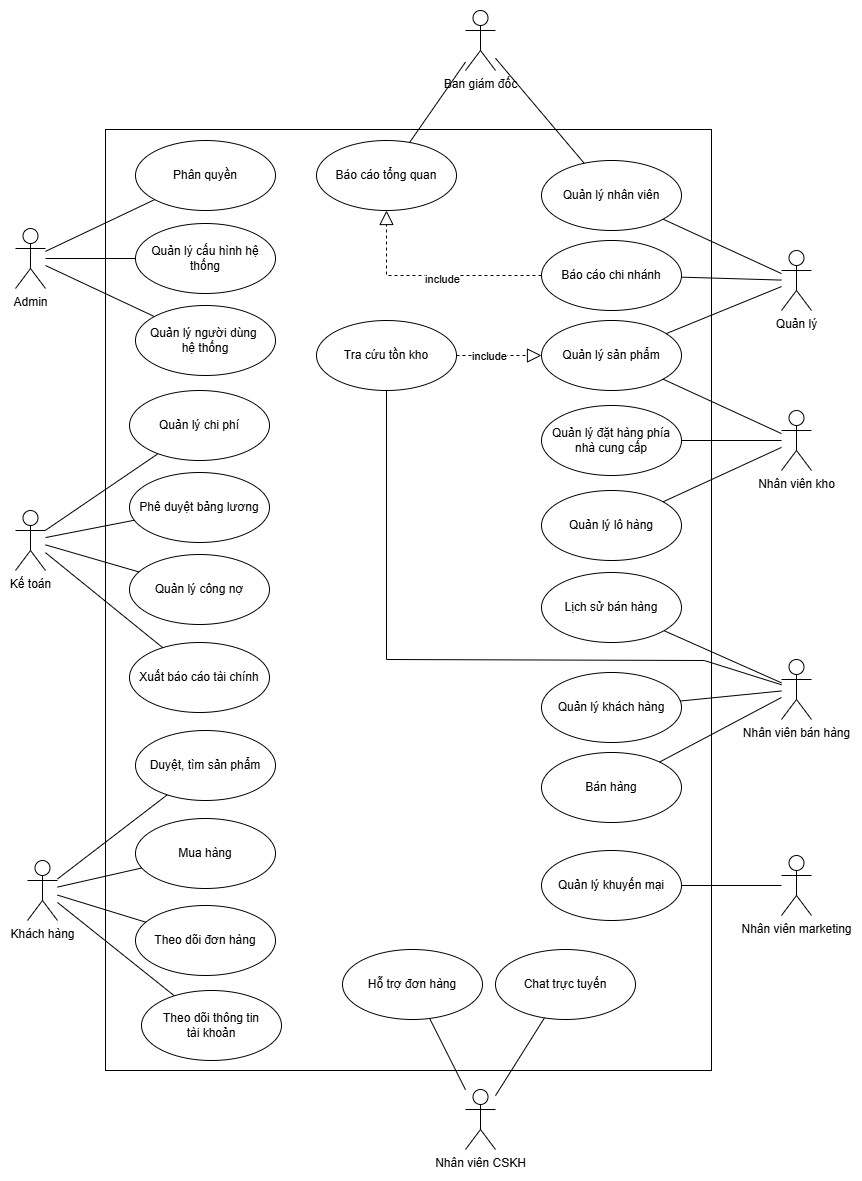
\includegraphics[width=0.72\textwidth]{VissoftIntern-Use_case.drawio.png}
\caption{Sơ đồ actor và use case tổng quát}
\label{fig:usecase}
\end{figure}

\chapter{Kiến trúc tổng thể}
\section{Mô hình triển khai}
Kiến trúc được tổ chức thành các lớp sau:
\begin{description}
  \item[Presentation] React SPA và storefront gửi REST request qua \texttt{/api}; chat dùng WebSocket.
  \item[Application] ASP.NET Core API tiếp nhận request, xác thực JWT, kiểm tra RBAC, validate DTO và gọi service nghiệp vụ.
  \item[Domain services] Pricing, inventory/FIFO, order, delivery, marketing, commission và reporting điều phối các quy tắc nghiệp vụ.
  \item[Persistence] PostgreSQL lưu dữ liệu chuẩn; EF Core/Dapper/Npgsql có thể được dùng theo loại truy vấn.
  \item[Infrastructure] Redis cung cấp cache-aside, invalidation, Pub/Sub và queue; worker xử lý job nền.
  \item[External integrations] Payment gateway, Google Maps, carrier API, Amazon SP-API và email service.
\end{description}

\begin{figure}[H]
\centering
\fbox{\begin{minipage}{0.92\textwidth}
\centering
React/Vite Frontend \(\longrightarrow\) ASP.NET Core Backend API \(\longrightarrow\) PostgreSQL 16\\[4pt]
\hfill\(\downarrow\) Redis cache/queue \hfill\(\downarrow\) External services
\end{minipage}}
\caption{Mô hình ba tầng và các điểm tích hợp}
\label{fig:architecture}
\end{figure}

\section{Nguyên tắc kiến trúc}
\begin{enumerate}
  \item Frontend không truy cập trực tiếp PostgreSQL hoặc PostgREST.
  \item PostgreSQL là nguồn dữ liệu chuẩn cho tồn, giá, trạng thái đơn, thanh toán và lợi nhuận.
  \item Logic nghiệp vụ nằm ở Backend service; database giữ constraint, khóa, transaction và dữ liệu bền vững.
  \item Redis không được quyết định giá hoặc tồn cuối cùng. Cache chỉ được cập nhật sau khi transaction PostgreSQL commit.
  \item Tác vụ nhiều bước dùng transaction; thao tác cạnh tranh dùng row-level locking hoặc optimistic locking.
  \item Tích hợp bên ngoài phải có timeout, retry giới hạn, idempotency và lưu trạng thái lỗi.
\end{enumerate}

\section{Công nghệ đề xuất}
\begin{table}[H]
\centering
\begin{tabularx}{\textwidth}{P{4.0cm}P{3.7cm}Y}
\toprule
Lớp & Công nghệ & Vai trò\\
\midrule
Frontend & React, TypeScript, Vite, Tailwind CSS & SPA, POS, storefront và giao diện responsive.\\
Backend & C\#, ASP.NET Core & API duy nhất, auth, RBAC, nghiệp vụ và WebSocket/SignalR.\\
Dữ liệu & PostgreSQL 16+ & Quan hệ, transaction, FK, unique, check và index.\\
Cache/queue & Redis 7.2 & Cache-aside, rate limit, Pub/Sub, job queue và realtime fan-out.\\
Data access & Npgsql, Dapper, EF Core & Truy cập dữ liệu quan hệ và báo cáo.\\
Tích hợp & Maps, carrier, payment, email, Amazon & Dịch vụ ngoại vi có kiểm soát.\\
Vận hành & Docker Compose, health/readiness & Khởi chạy và kiểm tra các service phụ thuộc.\\
\bottomrule
\end{tabularx}
\caption{Tech stack và vai trò}
\end{table}

\chapter{Phân tích nghiệp vụ và quy tắc cốt lõi}
\section{Catalog và biến thể}
Category được tổ chức theo cây, có thể dùng slug để truy vấn. Mỗi category có thể có badge riêng và được gán cho promotion hoặc combo.

Sản phẩm được mô hình hóa theo quan hệ sản phẩm cha--biến thể. Sản phẩm cha chứa tên, mô tả, category, ảnh và video. Biến thể chứa SKU, barcode, thuộc tính như size, màu, chất liệu, trọng lượng, CBM, số box và kích thước. Cách tách này cho phép mỗi biến thể có tồn, giá, lô và chính sách riêng trong khi vẫn hiển thị chung trên storefront.

Giá của biến thể được lưu theo lô. Lô này liên kết với một đơn đặt hàng từ nhà cung cấp. Giá nhập hàng của lô tương ứng với giá theo đơn đặt hàng này. Khi nhập về kho, lô được gán giá bởi quản lý hoặc được sinh tự động theo phần trăm lợi nhuận mục tiêu (quản lý sẽ là người thiết lập). Việc định giá theo lô cho phép tính lợi nhuận thực tế chính xác theo từng lô, phù hợp trong trường hợp giá nhập hàng thay đổi theo thời gian hoặc theo từng đơn đặt hàng.

Các bộ lọc nghiệp vụ gồm category, SKU, thuộc tính biến thể, khoảng giá, tình trạng còn hàng, hàng sắp về, shop và khoảng thời gian ETA. Catalog cũng hỗ trợ product association và combo để gợi ý các bộ sản phẩm phù hợp.

\section{Định giá năm giai đoạn}
Mỗi lô FIFO có \texttt{current\_stage} từ 1 đến 5 và một bảng giá riêng. Lô mới nhận được xếp \texttt{QUEUED}; lô đang bán là \texttt{ACTIVE}. Khi lô active hết hàng, backend đóng lô cũ, kích hoạt lô tiếp theo và reset giá về stage 1.

Tỷ lệ tồn bán được được tính theo:
\[
  \text{StockPercent} =
  \frac{\text{remaining quantity}}{\text{reference sellable quantity}}
  \times 100\%.
\]
Worker chạy định kỳ một lần mỗi ngày, ghi audit và invalidate cache sau commit.
Một stage chỉ chuyển khi đạt điều kiện tồn kho và thời gian tối thiểu; nếu vượt thời gian tối đa, stage chuyển để kích cầu dù tỷ lệ tồn chưa đạt ngưỡng. 

Việc chỉ thực hiện chuyển stage vào cuối ngày, không chuyển ngay khi hết lô là để tránh tình trạng giá thay đổi liên tục trong ngày, gây nhầm lẫn cho khách hàng và nhân viên bán hàng. Ví dụ trong 2 trường hợp sau:
\begin{itemize}
  \item Trường hợp 1: lô A còn 5 sản phẩm, lô B còn 10 sản phẩm. Lô A hết hàng lúc 10:00, lô B hết hàng lúc 15:00. Nếu chuyển stage ngay khi lô A hết, giá sẽ thay đổi vào lúc 10:00, nhưng sau đó lại thay đổi 1 lần nữa khi lô B hết hàng lúc 15:00. Khách hàng sẽ thấy giá thay đổi nhiều lần trong ngày.
  \item Trường hợp 2: lô A còn 5 sản phẩm, lô B còn 10 sản phẩm. Khách hàng mua 6 sản phẩm. Nếu chuyển stage ngay khi lô A hết, đơn hàng sẽ phải tính 5 sản phẩm giá cũ và 1 sản phẩm giá mới, gây nhầm lẫn cho khách hàng và nhân viên bán hàng. Nếu chuyển stage vào cuối ngày, tất cả các sản phẩm trong đơn hàng sẽ được tính giá theo stage cũ, tránh nhầm lẫn.
\end{itemize}

Quy trình chuyển stage được minh họa trong Hình \ref{fig:stage}.
\begin{figure}[H]
\centering
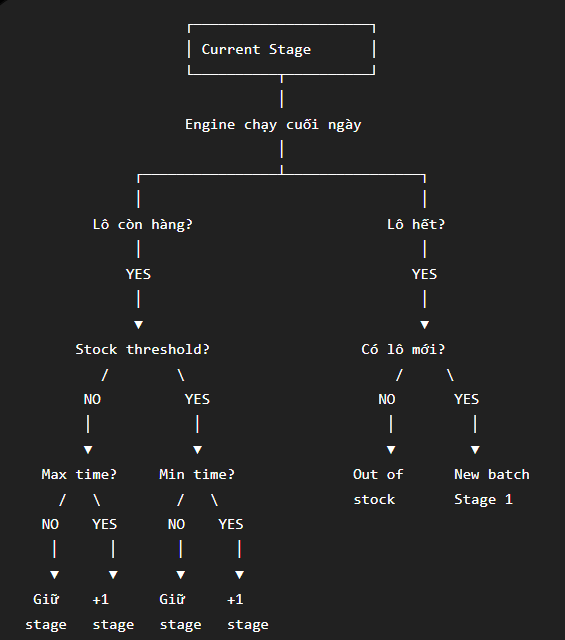
\includegraphics[height=0.72\textheight]{stage_transition.png}
\caption{Quy trình kiểm tra và chuyển stage giá}
\label{fig:stage}
\end{figure}

\section{POS, reservation và order lifecycle}
\begin{table}[H]
\centering
\begin{tabularx}{\textwidth}{P{3.2cm}Y Y}
\toprule
Loại đơn & Nguồn cấp hàng & Tác động chính\\
\midrule
Order Now & Lô active hiện tại & Khóa tồn, tăng reserved; khi giao thì outbound và chốt actual profit.\\
Pre-order & Container/lô tương lai đã chọn & Giữ chỗ nguồn hàng tương lai, không giảm on-hand hiện tại; khi nhập thì gán lô thực tế.\\
Future Delivery & Lô phù hợp với ngày hẹn & Giữ reservation theo kế hoạch và kiểm tra lại capacity tại thời điểm chuẩn bị giao.\\
\bottomrule
\end{tabularx}
\caption{Các loại đơn và tác động tồn kho}
\end{table}

Đơn hàng đi qua các trạng thái Draft, Pending, Processing, Shipping, Completed, Cancelled và Returned/Refunded. Chỉ Store Manager hoặc Super Admin được sửa các trường nhạy cảm sau khi tạo; mọi thay đổi cần audit log.

\section{Landed cost và điểm đặt hàng lại}
Với container có tổng cước và tổng CBM, chi phí vận chuyển trên mỗi CBM và landed cost được tính như sau:
\[
  \text{FreightPerCBM} =
  \frac{\text{Container freight}}{\text{Total CBM}},
\]
\[
  \text{LandedCost} =
  \text{Unit cost converted to AUD}
  + \text{Unit CBM}\times\text{FreightPerCBM}
  + \text{Customs and fees}.
\]
Giá stage 1 có thể được suy ra từ margin mục tiêu:
\[
  \text{Stage1Price} =
  \frac{\text{LandedCost}}{1-\text{TargetMargin}}.
\]
Từ stage 1, hệ thống sinh stage 2--5 theo tỷ lệ giảm mặc định và cho phép chỉnh trước khi áp dụng.

Điểm đặt hàng lại dựa trên vận tốc bán và lead time:
\[
  D = \frac{\text{quantity sold in last 30 days}}{30},
  \qquad
  \text{ROP}=D\times\text{LeadTime}+\text{SafetyStock}.
\]
Cảnh báo được tạo khi tồn thực tế cộng hàng đang về không vượt quá ROP.

\section{FIFO và lợi nhuận thực tế}
Lợi nhuận tại thời điểm tạo đơn chỉ là dự kiến. Khi hàng được xuất giao, backend phân bổ lô theo thứ tự \texttt{received\_date} tăng dần, lấy landed cost thực tế và tính:
\[
  \text{ActualProfit} =
  \text{Net sales} - \text{Actual FIFO cost} - \text{applicable costs}.
\]
Hủy đơn điều chỉnh lợi nhuận về 0 và giải phóng reservation. Đổi hàng tạo adjustment theo sản phẩm/lô mới. Commission chỉ chốt với đơn đã giao thành công.

\section{Delivery}
Delivery booking gắn với order và địa chỉ giao hàng. Calendar hỗ trợ Hour, Day, Week và Month view; mỗi booking có thể chứa yêu cầu lắp ráp, vác cầu thang, khung giờ và phụ phí. Dispatcher chọn các booking, backend chuẩn hóa tọa độ, gọi dịch vụ bản đồ để sắp xếp stop, rồi lưu route và stop.

Vòng đời stop gồm Prepare, Shipping, Done và Comeback. Chỉ khi stop Done và đủ allocation thực tế, order mới được Completed và lợi nhuận FIFO mới được chốt. Comeback tạo quy trình quay hàng/kiểm tra thay vì ghi nhận giao thành công.

\section{Marketing, loyalty và commission}
Promotion hỗ trợ giảm theo phần trăm hoặc số tiền, thời gian hiệu lực, badge và product/combo mapping. Nếu promotion phụ thuộc phần trăm giá gốc, giá sale phải thay đổi theo giá stage mới.

Khách hàng được tích điểm theo chính sách, có thể được gán VIP thủ công. Nếu có VIP price riêng thì ưu tiên giá đó; nếu không, khách VIP được hưởng stage ưu đãi sớm hơn một mức, nhưng không cộng chồng nhiều ưu đãi.

Với định mức doanh số theo giờ, commission được tính theo:
\[
  \text{TargetSales}=\text{HoursWorked}\times\text{SalesPerHourTarget},
\]
\[
  \text{GrossCommission}=\max(0,\text{ActualCompletedSales}-\text{TargetSales})
  \times\text{CommissionRate}.
\]
Các điều chỉnh do hủy hoặc đổi phải được phản ánh vào kỳ commission tương ứng.

\chapter{Thiết kế dữ liệu}
\section{Các miền dữ liệu}
Danh mục thực thể dưới đây được đối chiếu theo tài liệu \texttt{DATABASE\_TABLES\_KEYS.md}; tên bảng và quan hệ được giữ theo data dictionary làm nguồn tham chiếu cho phần thiết kế dữ liệu.
\begin{table}[H]
\centering
\begin{tabularx}{\textwidth}{P{3.8cm}Y}
\toprule
Miền & Thực thể tiêu biểu\\
\midrule
Core và RBAC & addresses, stores, users, roles, user\_roles, warehouses, store\_warehouses, postcodes, postcode\_stores, store\_shipping\_rates.\\
Catalog và pricing & product\_categories, products, product\_variants, fifo\_lot\_stage\_prices, pricing\_stage\_configs, store\_variant\_prices, stage\_price\_audit\_logs.\\
Supply chain & suppliers, stock\_orders, stock\_order\_items, fifo\_lots.\\
Inventory & warehouse\_inventory, inventory\_transactions, inventory\_transfers, inventory\_transfer\_items.\\
CRM và order & customers, customer\_loyalty\_transactions, orders, order\_items, order\_payments, order\_audit\_logs, order\_item\_fifo\_allocations.\\
Delivery & carriers, drivers, delivery\_bookings, delivery\_routes, delivery\_stops.\\
Marketing và finance & promotions, promotion\_products, product\_combos, combo\_items, product\_associations, ad\_spend\_logs, sales\_shifts, sales\_commissions.\\
Chat & chat\_sessions, chat\_messages.\\
\bottomrule
\end{tabularx}
\caption{Nhóm thực thể và trách nhiệm dữ liệu}
\end{table}

\section{Mô hình persistence và data dictionary}
Thiết kế database dùng PostgreSQL 16+ làm nguồn dữ liệu bền vững duy nhất. Database chịu trách nhiệm lưu trữ, quan hệ, kiểu dữ liệu, khóa, chỉ mục và các constraint an toàn như \texttt{NOT NULL}, \texttt{UNIQUE} và kiểm tra giá trị không âm. Logic FIFO, chuyển stage giá, phân bổ tồn, tính commission, RBAC và audit workflow được thực hiện tại Backend Application; không đưa business logic vào stored trigger hoặc stored procedure phức tạp.

\begin{figure}[H]
\centering
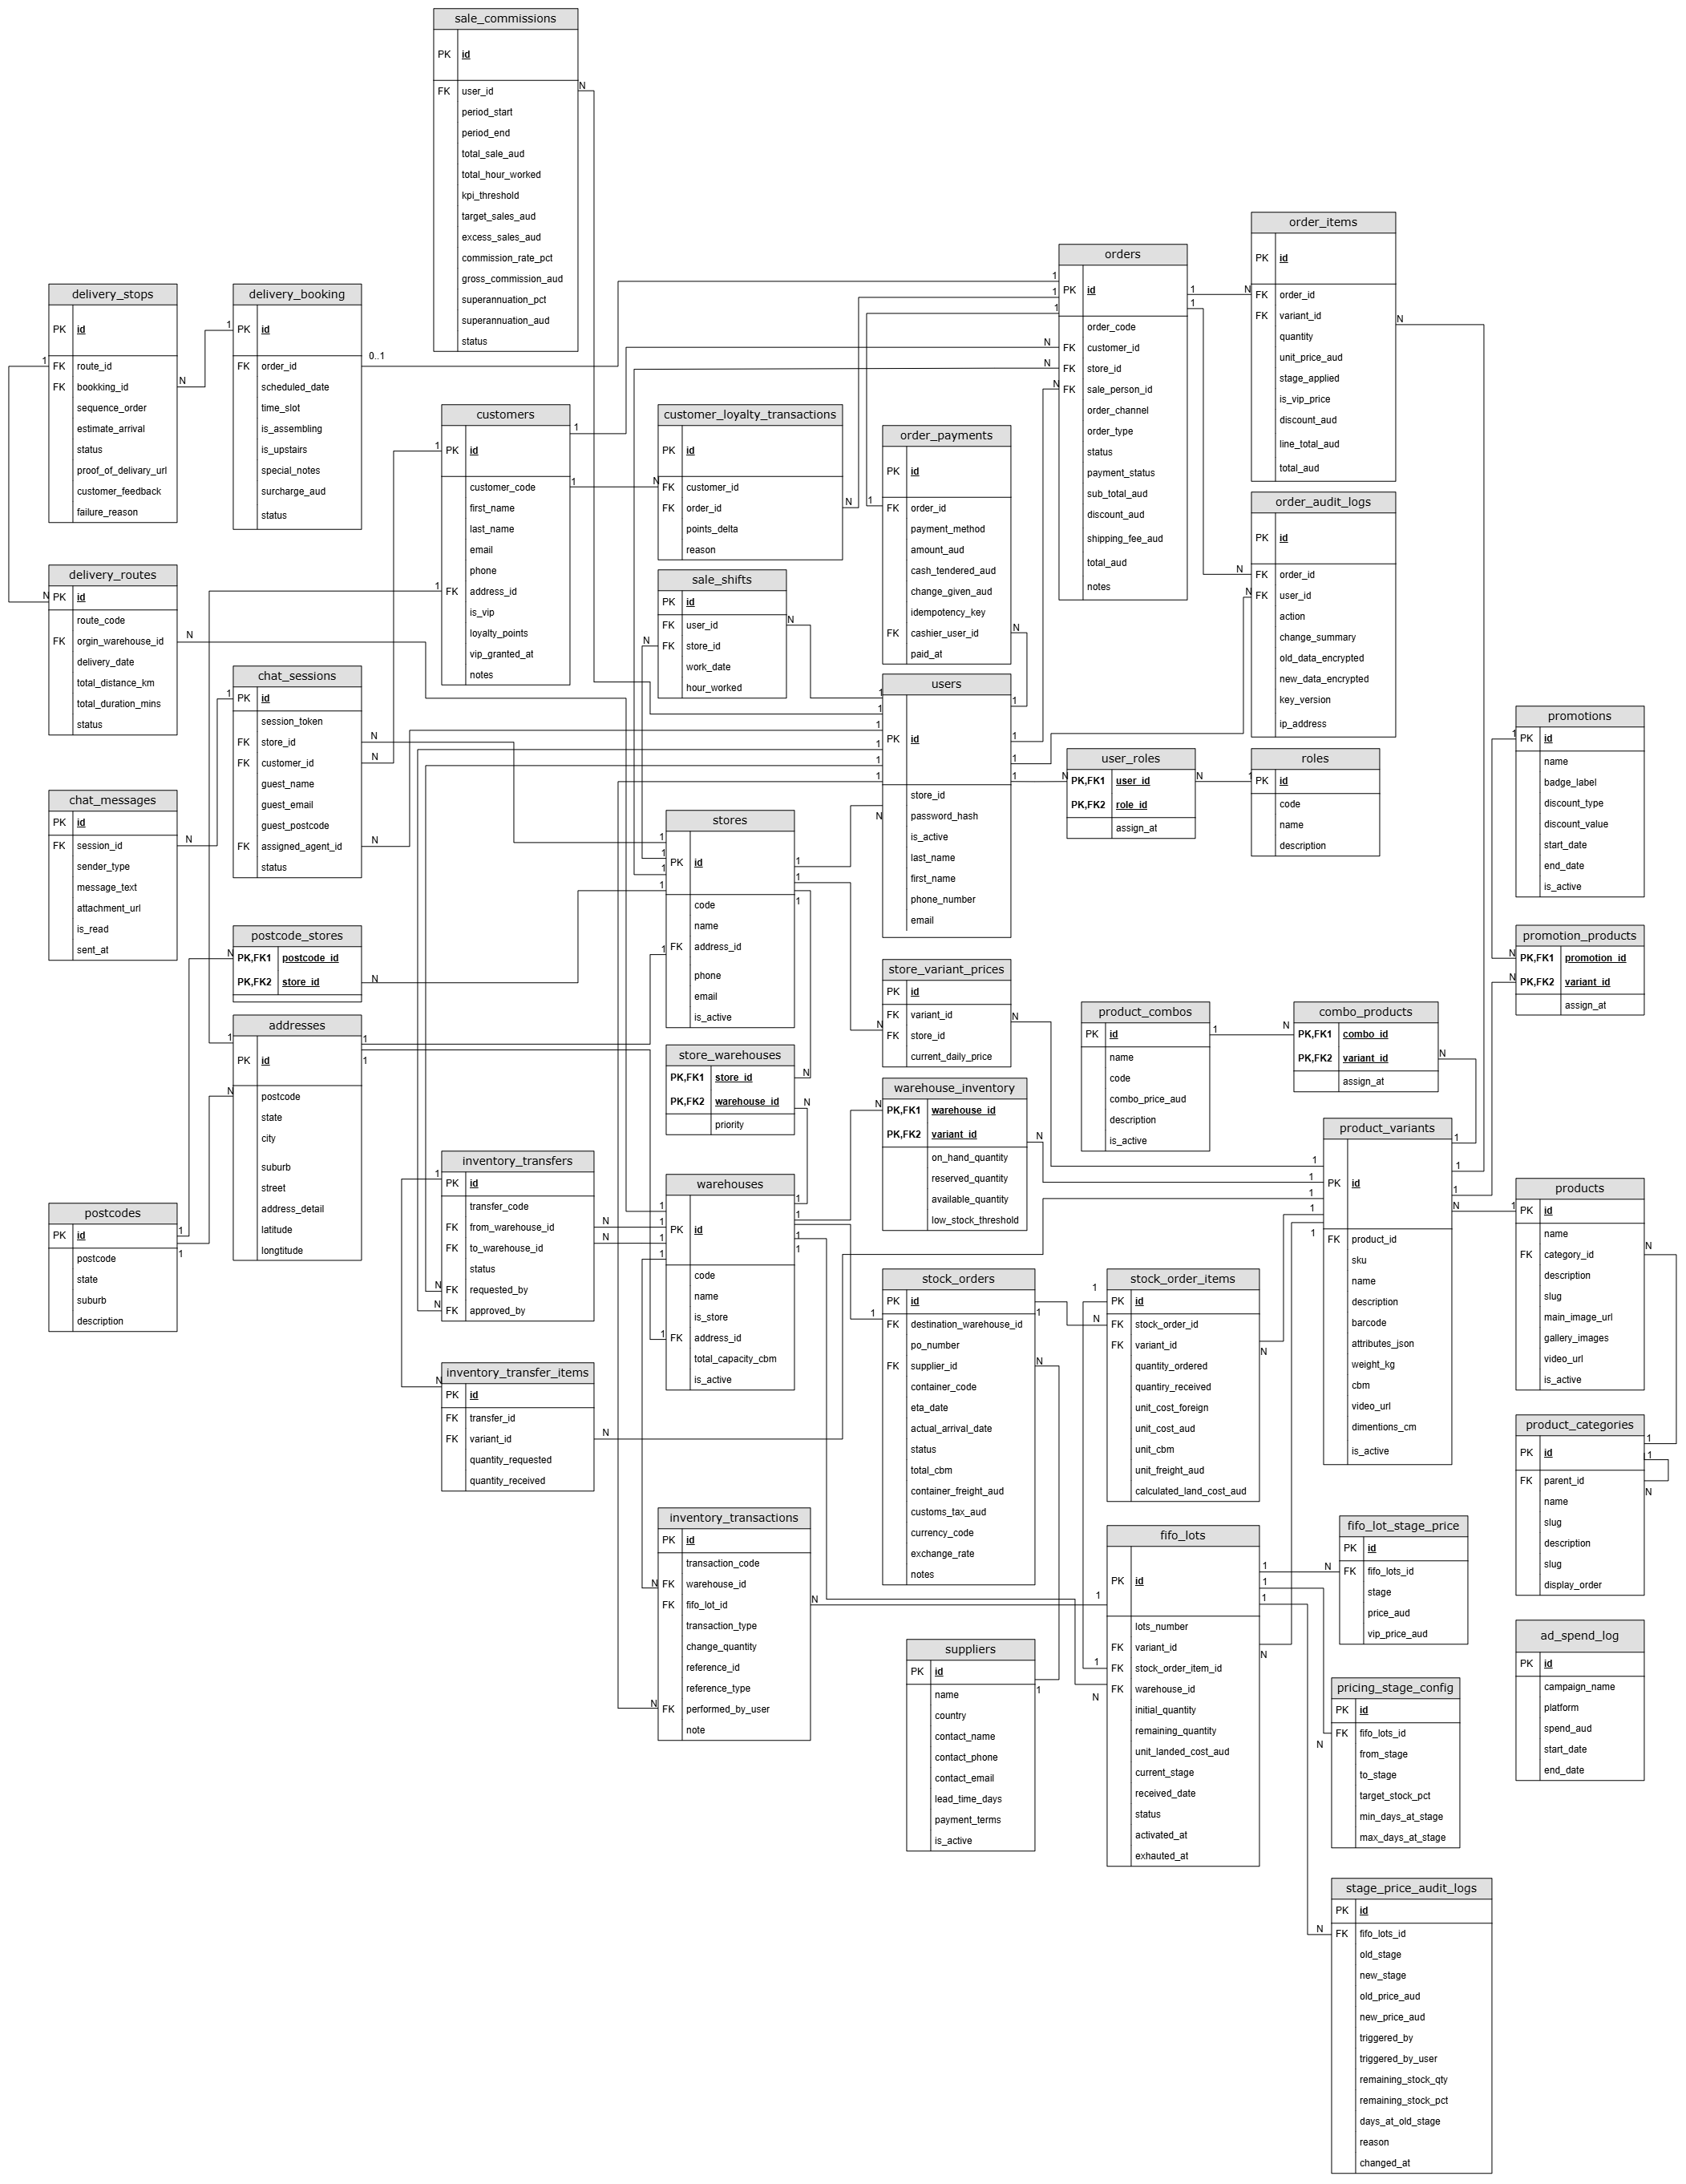
\includegraphics[width=\textwidth]{../design/VissoftIntern-DB.drawio.png}
\caption{ERD của hệ thống quản lý bán hàng theo mô hình đa chi nhánh}
\label{fig:erd-main}
\end{figure}


\section{ERD logic và các quan hệ trung tâm}

\begin{figure}[H]
\centering
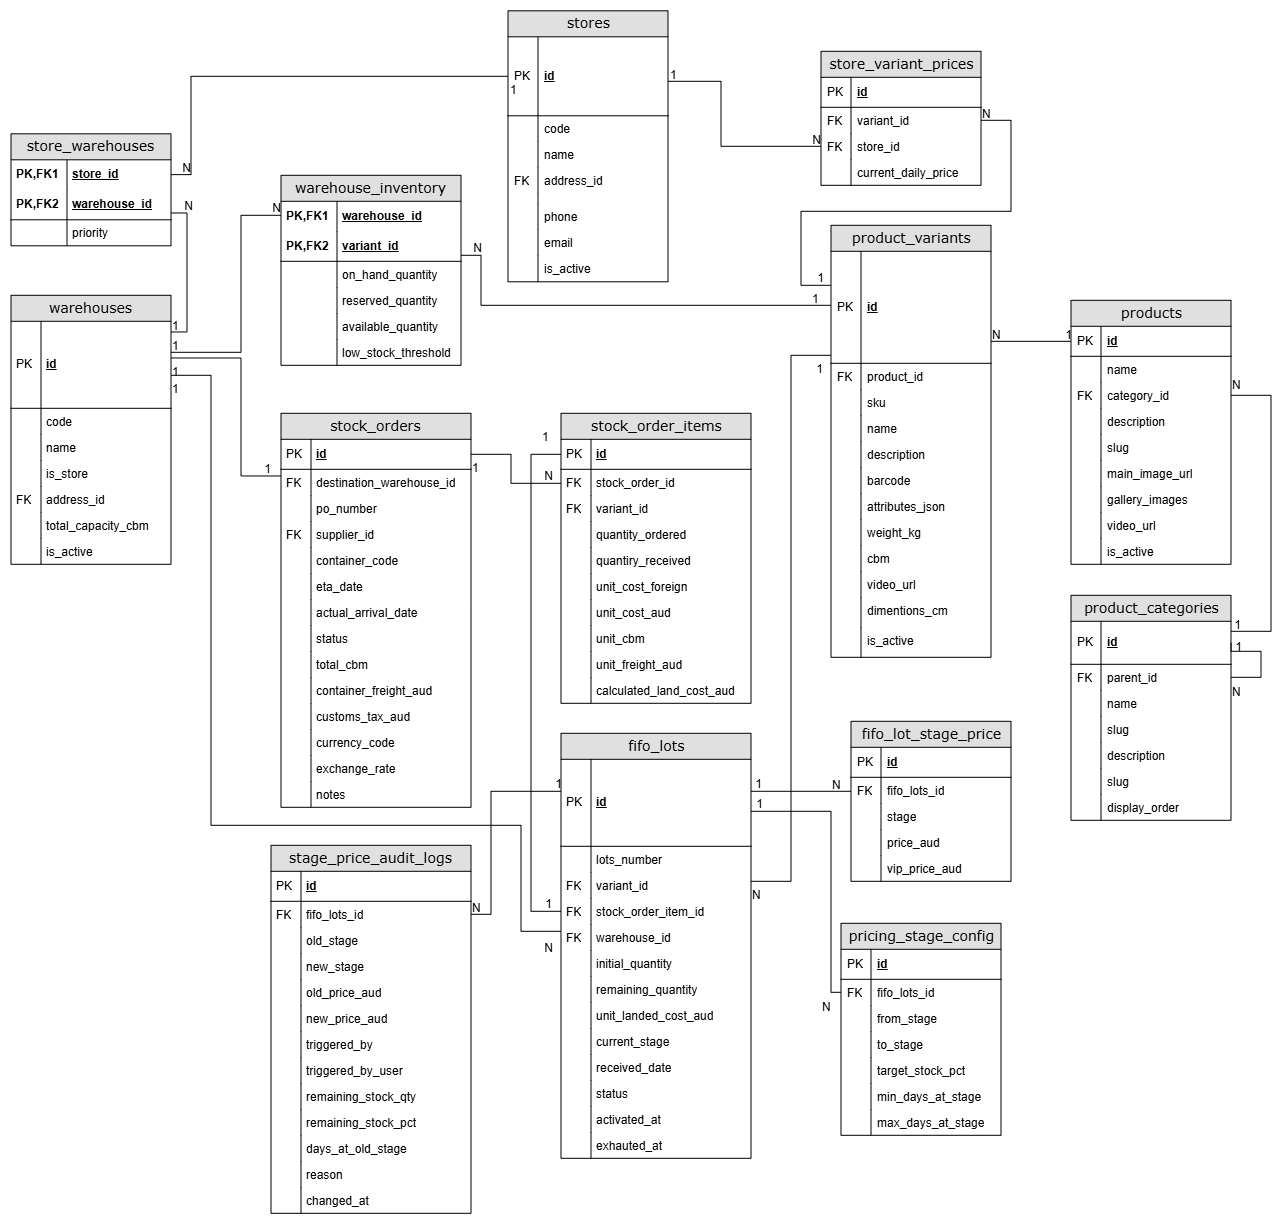
\includegraphics[width=0.92\textwidth]{../design/VissoftIntern-Price_engine_Exclude_unrelated.drawio.png}
\caption{Các bảng lưu trữ dữ liệu giá sản phẩm và phục vụ tính giá theo 5 stage của price engine}
\label{fig:price-engine-tables}
\end{figure}

\begin{sloppypar}
Catalog đi theo chuỗi \texttt{products} $\rightarrow$ \texttt{product\_variants} $\rightarrow$ \texttt{fifo\_lots}; mỗi lot liên kết với \texttt{stock\_order\_items}, tồn kho và bảng giá stage. Các combo được biểu diễn qua \texttt{product\_combos} và \texttt{combo\_items}.
Khuyến mại sản phẩm dùng \texttt{promotion\_products}.
\end{sloppypar}

\begin{figure}[H]
\centering
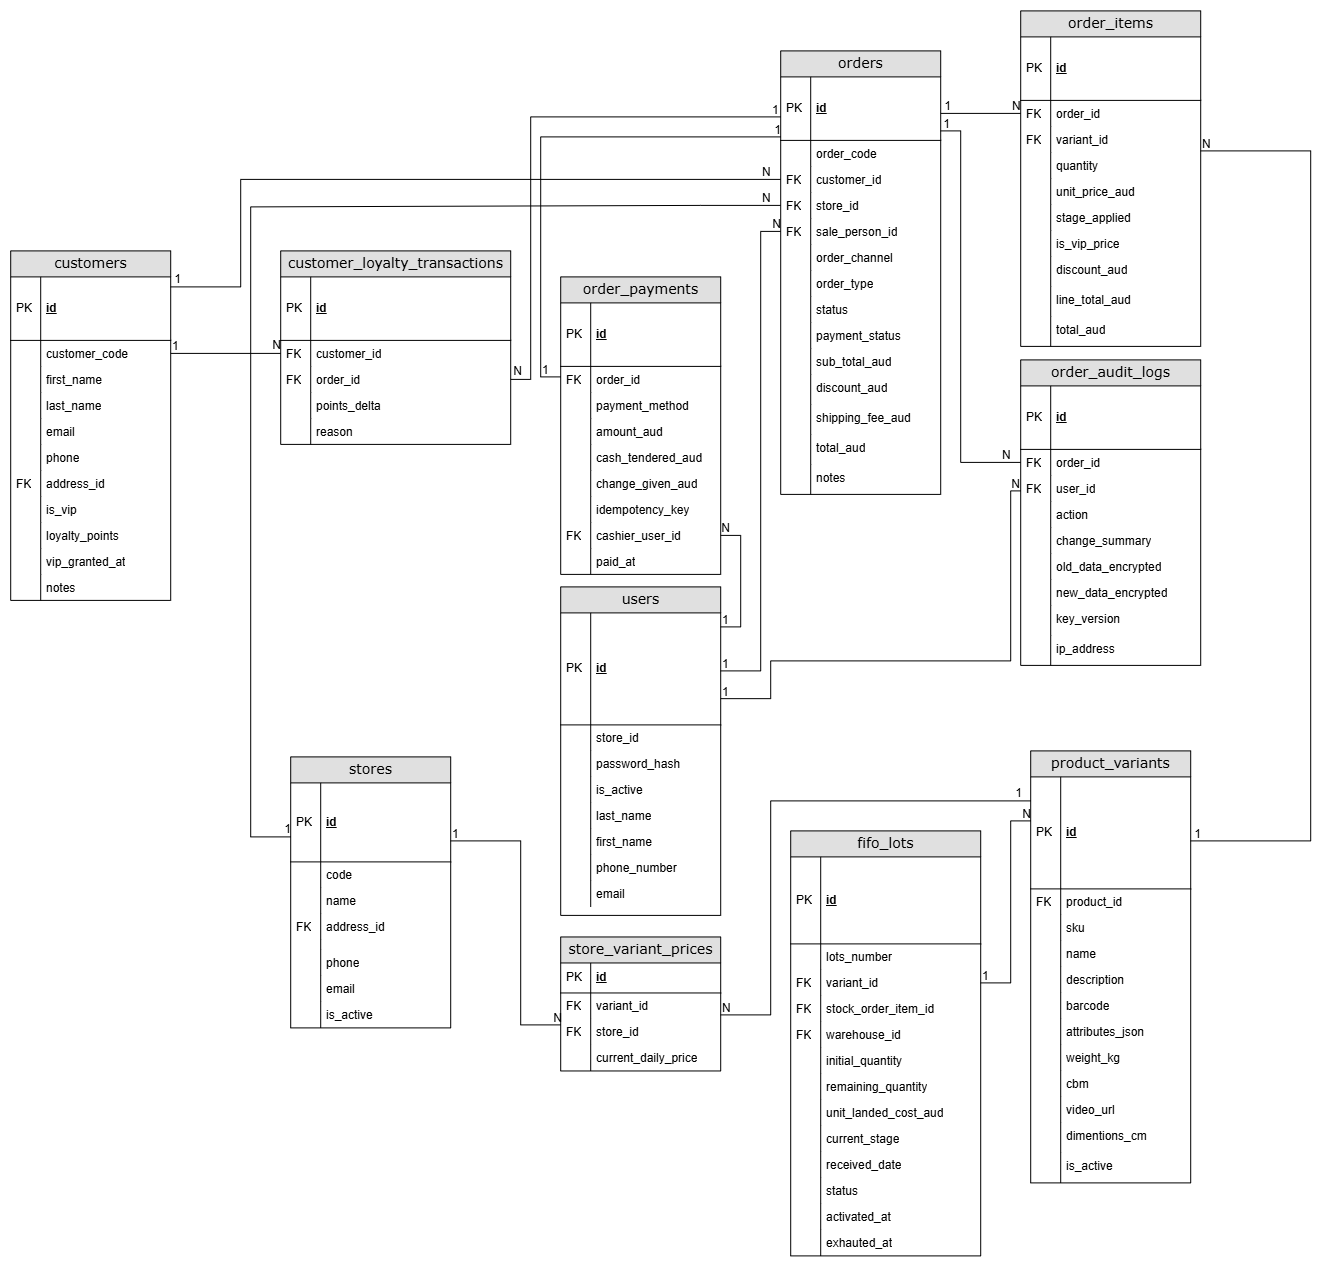
\includegraphics[width=0.92\textwidth]{../design/VissoftIntern-Sale_and_price_cal_Exclude_unrelated.drawio.png}
\caption{Các bảng lưu trữ dữ liệu đơn hàng, payment và phân bổ FIFO}
\label{fig:sale-price-tables}
\end{figure}


Đơn hàng nối khách hàng, cửa hàng, các dòng hàng, payment và allocation FIFO. 

\begin{figure}[H]
\centering
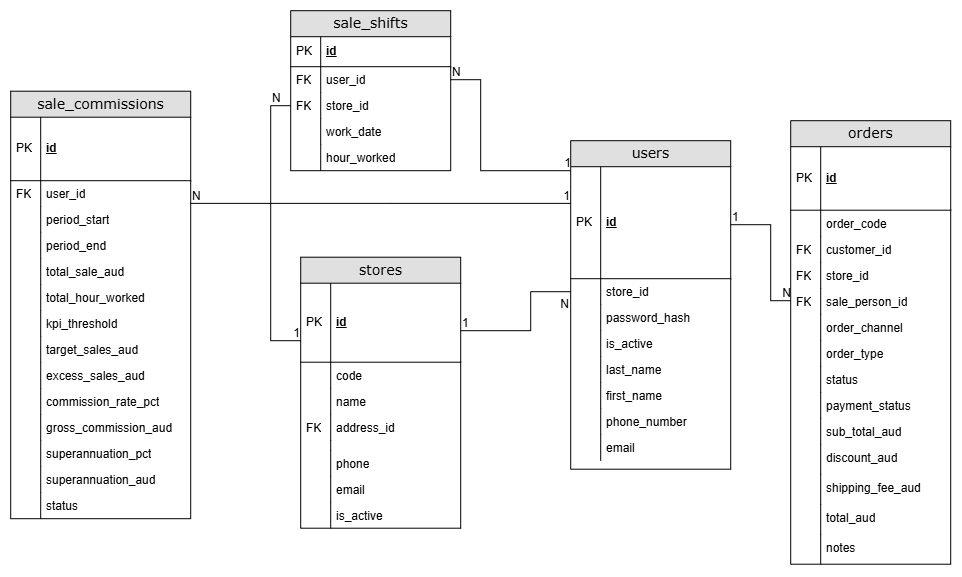
\includegraphics[width=0.92\textwidth]{../design/VissoftIntern-Superannual_exclude_unrelated.drawio.png}
\caption{Các bảng lưu trữ dữ liệu tính commission của nhân viên bán hàng}
\end{figure}

Delivery nối đơn hàng với booking, route, stop, carrier và driver. 
Promotion, combo, loyalty, commission và chat là các miền mở rộng dùng khóa ngoại để giữ traceability.

\begin{table}[H]
\centering
\begin{tabularx}{\textwidth}{P{4.1cm}Y}
\toprule
Quan hệ & Bất biến thiết kế\\
\midrule
Store -- Warehouse & Nhiều-nhiều qua \path{store_warehouses}; \path{priority} lớn hơn 0 để chọn nguồn cấp hàng.\\
Product -- Variant & Một product có nhiều variant; SKU và barcode của variant phải duy nhất.\\
Variant -- FIFO Lot & Lot thuộc một variant và một warehouse; \path{remaining_quantity} không vượt \path{initial_quantity}.\\
Warehouse -- Inventory & Khóa ghép warehouse/variant; reserved không được vượt on-hand và available không âm.\\
Order -- Payment & Mỗi payment có idempotency key; transaction reference không được trùng khi có giá trị.\\
Order Item -- FIFO Allocation & Một dòng hàng có thể phân bổ nhiều lot; realized profit dùng landed cost của từng lot.\\
Order -- Delivery & Booking lưu lịch giao; stop Done mới cho phép hoàn tất đơn và chốt lợi nhuận.\\
Store -- Shipping Rate & Cùng một cửa hàng không được có các khoảng distance bị overlap.\\
\bottomrule
\end{tabularx}
\caption{Các quan hệ và bất biến quan trọng}
\end{table}

\section{Quan hệ và khóa}
\begin{sloppypar}
\raggedright
Các bảng danh mục dùng khóa chính dạng \texttt{BIGSERIAL}; bảng nối nhiều-nhiều như \texttt{store\_warehouses}, \texttt{postcode\_stores}, \texttt{promotion\_products} và \texttt{product\_associations} dùng khóa ghép. Foreign key được dùng cho các quan hệ giữa store, warehouse, product, order, lot, delivery và chat. Constraint \texttt{CHECK} bảo vệ các đại lượng không âm, stage trong khoảng 1--5, số lượng còn lại không vượt số lượng ban đầu, reserved không vượt on-hand và khoảng cách vận chuyển hợp lệ.
\end{sloppypar}

Các index quan trọng gồm index theo SKU, slug, product/category, trạng thái và ETA của stock order, lot theo variant--warehouse--status, inventory theo warehouse--variant, order theo trạng thái/ngày, route theo delivery date, chat theo session/time và audit theo entity/time. Extension \texttt{pg\_trgm} hỗ trợ tìm kiếm tên/SKU; \texttt{btree\_gist} kết hợp exclusion constraint để ngăn khoảng cách cước của cùng một store bị chồng lấn.

\section{Nguyên tắc toàn vẹn dữ liệu}
\begin{enumerate}
  \item Một payment request phải có idempotency key hoặc gateway reference duy nhất.
  \item Cập nhật on-hand, reserved, allocation và inventory transaction phải nằm trong cùng transaction.
  \item Một biến thể chỉ có một giá ngày cho một cửa hàng tại một thời điểm.
  \item Lô exhausted không được tiếp tục cấp hàng; lô queued chỉ được active theo quy tắc FIFO.
  \item Dữ liệu audit phải chứa actor, entity, hành động, before/after, thời điểm và request context.
  \item Xóa dữ liệu nghiệp vụ cần tôn trọng \texttt{ON DELETE RESTRICT} ở các bảng có ảnh hưởng tài chính hoặc tồn kho.
\end{enumerate}

\chapter{Thiết kế API và giao tiếp}
\section{Quy ước API}
API dùng JSON và response envelope thống nhất:
\begin{lstlisting}
{
  "success": true,
  "data": { },
  "meta": { "page": 1, "limit": 20, "total": 125, "totalPages": 7 }
}
\end{lstlisting}
Danh sách hỗ trợ \texttt{page} và \texttt{limit}, trong đó \texttt{limit} có giới hạn tối đa. Request nội bộ dùng Bearer token; storefront public chỉ mở khóa giá và checkout sau khi resolve postcode. Lỗi vượt rate limit trả HTTP 429 kèm retry information.

\section{Bề mặt endpoint theo phân hệ}
\begin{longtable}{P{3.0cm}P{5.0cm}P{6.0cm}}
\toprule
Phân hệ & Endpoint tiêu biểu & Chức năng\\
\midrule
Auth & \path{/api/auth/login}, \path{/api/auth/me} & Đăng nhập, profile và role.\\
Stores & \path{/api/stores}, \path{/api/warehouses}, \path{/api/postcodes/lookup} & Cửa hàng, kho và mapping postcode.\\
Catalog & \path{/api/categories}, \path{/api/products}, \path{/api/products/price-stage-check} & Sản phẩm, biến thể, giá và worker stage.\\
Supply & \path{/api/suppliers}, \path{/api/stock-orders}, \path{/api/stock-orders/landed-cost} & NCC, container, landed cost và nhận hàng.\\
Inventory & \path{/api/inventory/stock}, \path{/api/inventory/fifo-lots}, \path{/api/inventory/transfers} & Tồn, lô và điều chuyển.\\
Orders & \path{/api/customers}, \path{/api/orders}, \path{/api/orders/:id/payments} & CRM, POS, thanh toán và audit.\\
Delivery & \path{/api/deliveries/calendar}, \path{/api/deliveries/routes}, \path{/api/deliveries/optimize-route} & Lịch, tuyến, stop và trạng thái giao.\\
Marketing & \path{/api/marketing/promotions}, \path{/api/marketing/combos}, \path{/api/reports/financial-pnl} & Promotion, combo, ads và P\&L.\\
Storefront & \path{/api/storefront/resolve-postcode}, \path{/api/storefront/products}, \path{/api/storefront/checkout} & Giá theo vùng, catalog và checkout.\\
Chat & \path{/api/chat/session}, WebSocket events & Session, message và typing.\\
\bottomrule
\caption{Các nhóm endpoint chính}\label{tab:api-groups}\\
\end{longtable}

\section{Các hợp đồng quan trọng}
\begin{sloppypar}
\raggedright
\begin{itemize}
  \item \api{POST /api/products/price-stage-check}: trả stage cũ/mới, giá cũ/mới và lý do chuyển.
  \item \api{POST /api/stock-orders/:id/receive}: tạo FIFO lot, cập nhật tồn và đối chiếu pre-order.
  \item \api{POST /api/orders}: tạo Order Now, Pre-order hoặc Future Delivery; backend tự lấy giá và tồn chuẩn.
  \item \api{PUT /api/deliveries/stops/:id/status}: khi Done sẽ outbound FIFO và chốt actual profit.
  \item \api{POST /api/storefront/resolve-postcode}: xác định store phục vụ, mở khóa giá và cung cấp rate cơ bản.
  \item WebSocket events gồm \texttt{join\_session}, \texttt{agent\_join}, \texttt{send\_message}, \texttt{receive\_message} và \texttt{typing}.
\end{itemize}
\end{sloppypar}

\chapter{Thiết kế luồng dữ liệu và xử lý đồng thời}
\section{Cache-aside}
Luồng đọc là API đọc Redis trước; cache miss thì đọc PostgreSQL và populate Redis. Luồng ghi luôn đi qua API, commit PostgreSQL trước rồi mới invalidate hoặc refresh cache. Các key hạt mịn được tổ chức theo entity, ví dụ:
\begin{itemize}
  \item \texttt{price:\{storeId\}:\{variantId\}:\{lotId\}} cho giá theo lô và cửa hàng;
  \item \texttt{stock:\{warehouseId\}:\{variantId\}} cho tồn khả dụng;
  \item \texttt{lot:active:\{warehouseId\}:\{variantId\}} cho lô active;
  \item \texttt{customer:loyalty:\{customerId\}} cho điểm khách hàng.
\end{itemize}
Không dùng xóa cache toàn cục cho thay đổi của một SKU.

\section{Luồng nhập container}
Nhân viên tạo stock order ở trạng thái draft. Khi nhận hàng, backend mở transaction, cập nhật số lượng thực nhận, tạo lot và bảng giá, tăng inventory, ghi inventory transaction, đối chiếu reservation, commit rồi invalidate cache. Thiếu hoặc hỏng hàng phải được ghi nhận rõ, không tự động cấp vượt số thực nhận.

\section{Luồng giao hàng và lợi nhuận}
Dispatcher chọn booking, backend tạo route/stop. Khi stop Done, backend khóa stop, order và allocation; tiêu thụ lot theo FIFO; ghi outbound; cập nhật on-hand/reserved; ghi audit; chuyển order Completed; tính actual FIFO profit; commit; sau đó mới phát job commission/report và invalidate cache.

\section{Xử lý lỗi}
\begin{table}[H]
\centering
\begin{tabularx}{\textwidth}{P{4.0cm}Y}
\toprule
Tình huống & Cách xử lý\\
\midrule
Deadlock hoặc lock timeout & Rollback, retry có backoff và giới hạn số lần.\\
Payment callback trùng & Deduplicate bằng gateway reference/idempotency key.\\
Maps/carrier timeout & Timeout ngắn, retry giới hạn, chuyển manual review nếu cần.\\
Redis lỗi & Đọc PostgreSQL; không ghi nghiệp vụ thay Redis.\\
Worker chạy lại & Dùng job key và audit deduplication.\\
Giao hàng thất bại & Chuyển Comeback, tạo return/inspection, không Completed.\\
\bottomrule
\end{tabularx}
\caption{Chiến lược lỗi và khôi phục}
\end{table}

\chapter{Phân tích thiết kế giao diện}
\section{Nguyên tắc giao diện storefront}
Wireframe mô tả một storefront có header cố định với logo, Home, About, Gallery, Blog, Contact, tìm kiếm, cart và login; nội dung được chia theo vùng rõ ràng với footer. Mục tiêu trải nghiệm là cho phép duyệt sản phẩm trước, nhưng chỉ hiển thị giá và cho phép thêm vào giỏ sau khi khách nhập postcode hợp lệ.

\begin{figure}[H]
\centering
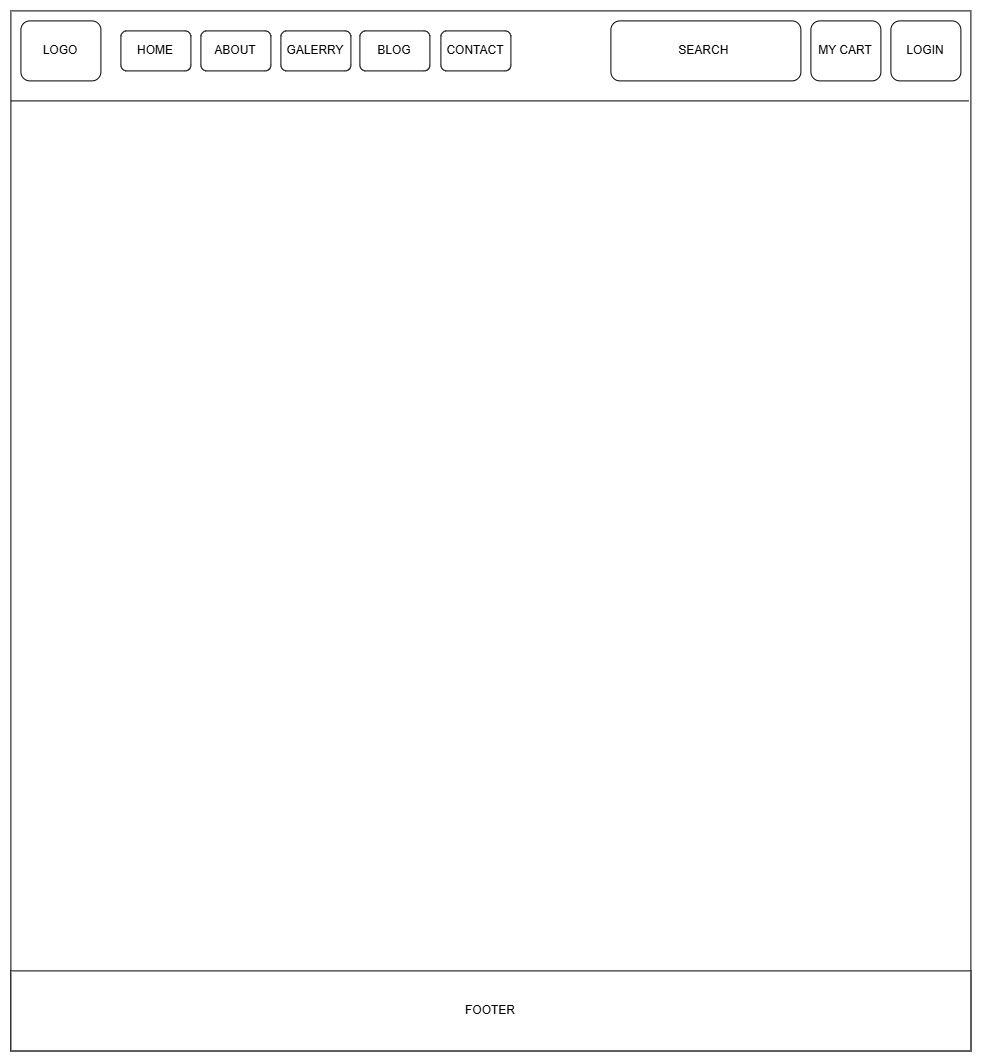
\includegraphics[width=0.70\textwidth]{VissoftIntern-Site_template.drawio.png}
\caption{Template bố cục website}
\label{fig:site-template}
\end{figure}

\section{Trang chủ và điều hướng catalog}
Trang chủ có banner, bốn nhóm chính Living Room, Dining Room, Bedroom, Outdoor \& Others, tiếp theo là các dải Most Purchased, Hottest Sale và Packages. Product card có hình ảnh và nút View Price; popup postcode là chốt mở khóa giá.

\begin{figure}[H]
\centering
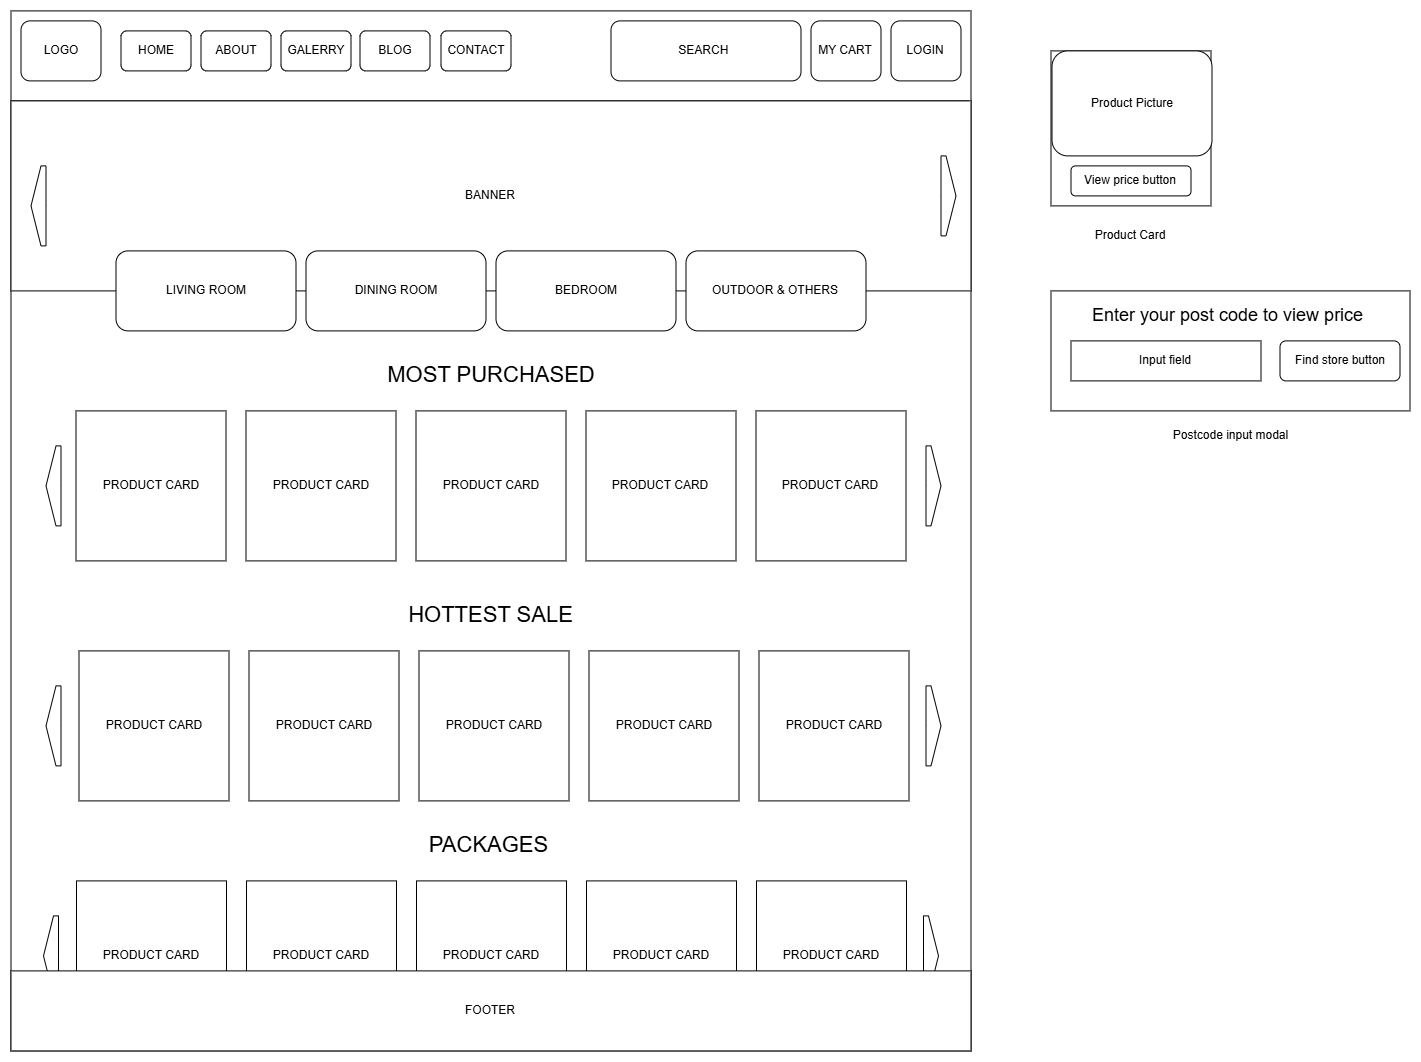
\includegraphics[width=0.91\textwidth]{VissoftIntern-HOME_UI.drawio.png}
\caption{Wireframe trang chủ và modal postcode}
\label{fig:home}
\end{figure}

\section{Trang danh mục}
Trang danh mục dùng bố cục hai vùng: sidebar chứa category, price range, brand, color, size và bộ lọc mở rộng; vùng chính là lưới product card có phân trang. Đây là điểm phù hợp để kết nối query filter, pagination và trạng thái giá theo store.

\begin{figure}[H]
\centering
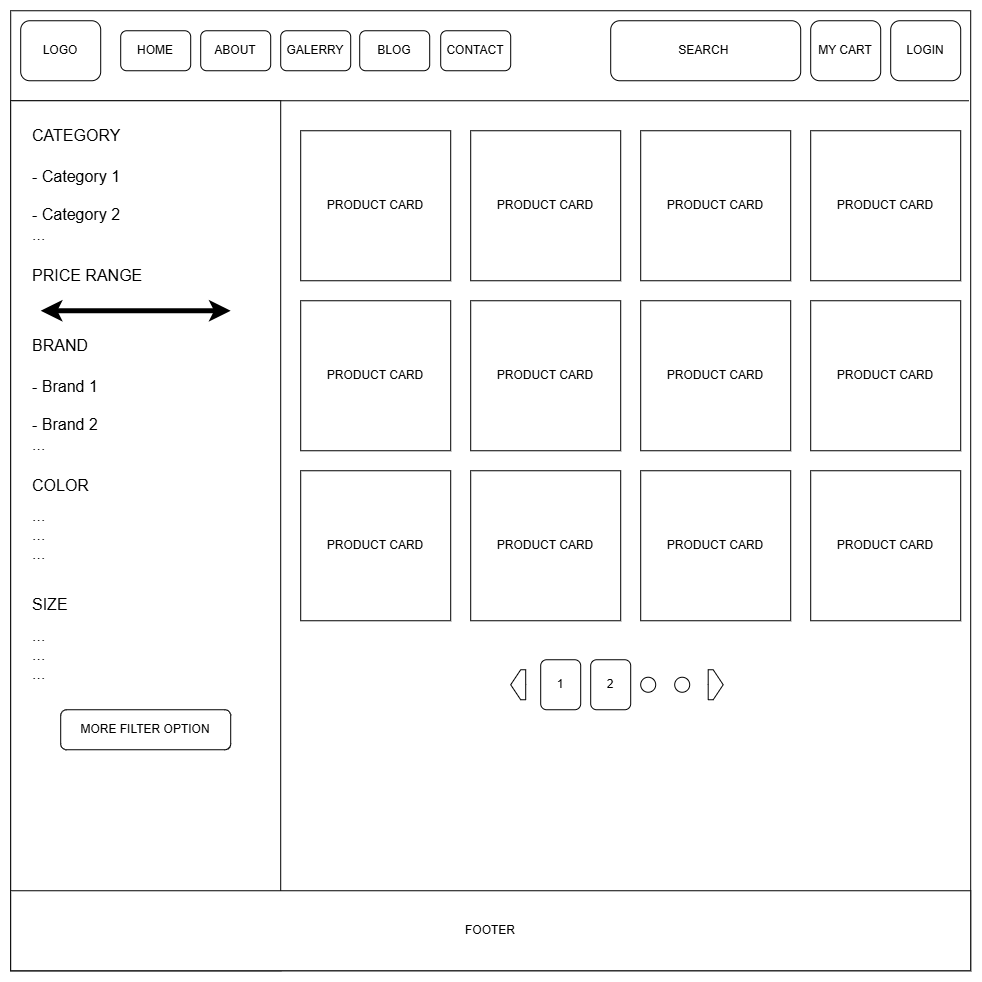
\includegraphics[width=0.91\textwidth]{VissoftIntern-SHOP_UI.drawio.png}
\caption{Wireframe trang danh mục và bộ lọc}
\label{fig:shop}
\end{figure}

\section{Trang chi tiết sản phẩm}
Trang chi tiết gồm gallery ảnh, tên sản phẩm, View Price, các lựa chọn color/material/size, bộ tăng giảm số lượng và Add to cart. Bên dưới là các tab Description, Specification và Reviews, tiếp theo là các product card liên quan. Từ góc nhìn domain, các lựa chọn variant phải được backend kiểm tra lại về giá, tồn và khả dụng trước khi thêm giỏ.

\begin{figure}[H]
\centering
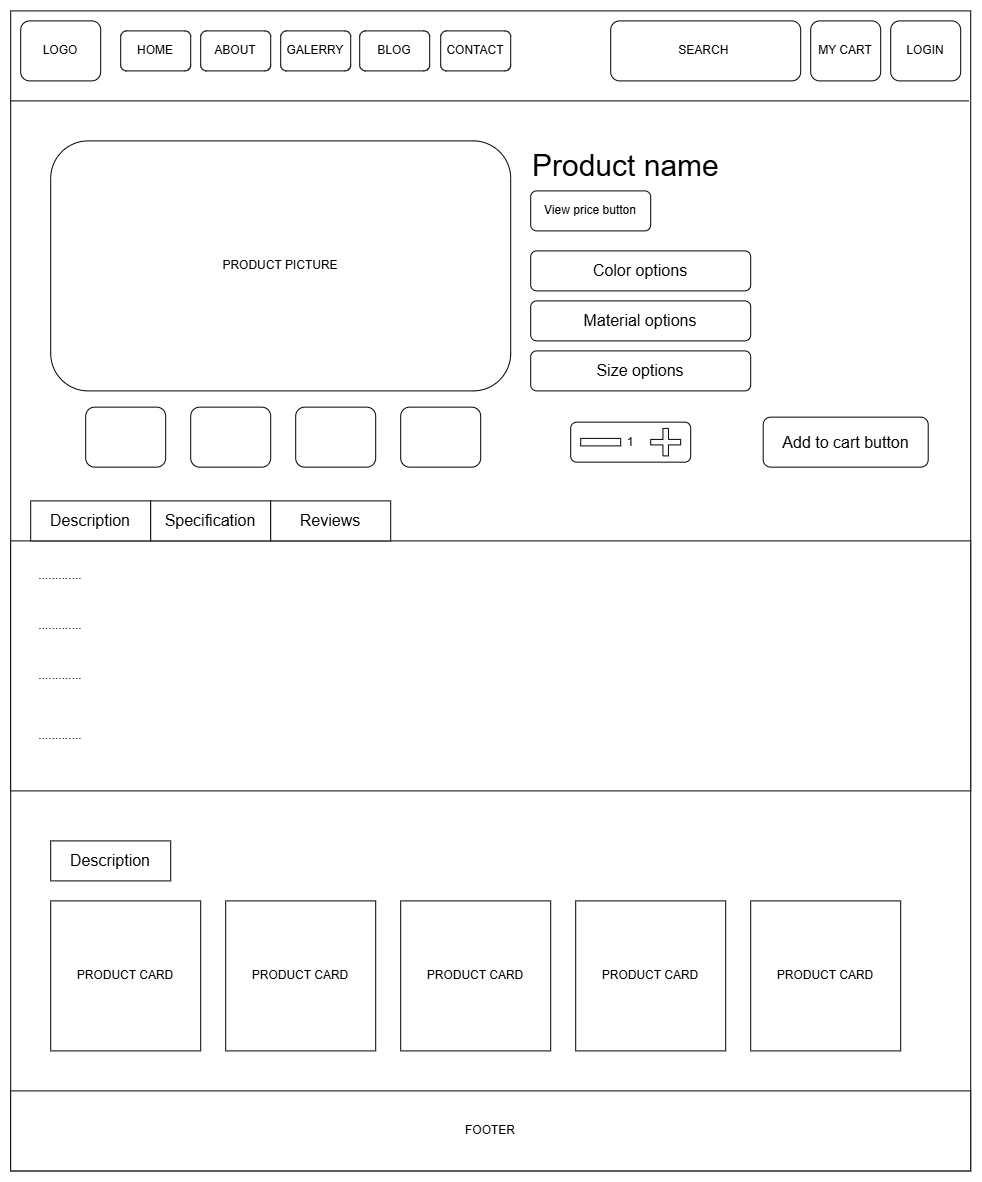
\includegraphics[width=0.91\textwidth]{VissoftIntern-PRODUCT_DETAIL.drawio.png}
\caption{Wireframe trang chi tiết sản phẩm}
\label{fig:product-detail}
\end{figure}

\section{Giỏ hàng}
Giỏ hàng hiển thị từng sản phẩm, ảnh, variant choice, số lượng, giá, checkbox chọn dòng và vùng tóm tắt promotion code, subtotal, shipping, discount và grand total. Giá gửi từ client không được xem là nguồn tin cậy; checkout phải resolve postcode, đọc giá hiện hành, promotion, VIP và tồn từ backend.

\begin{figure}[H]
\centering
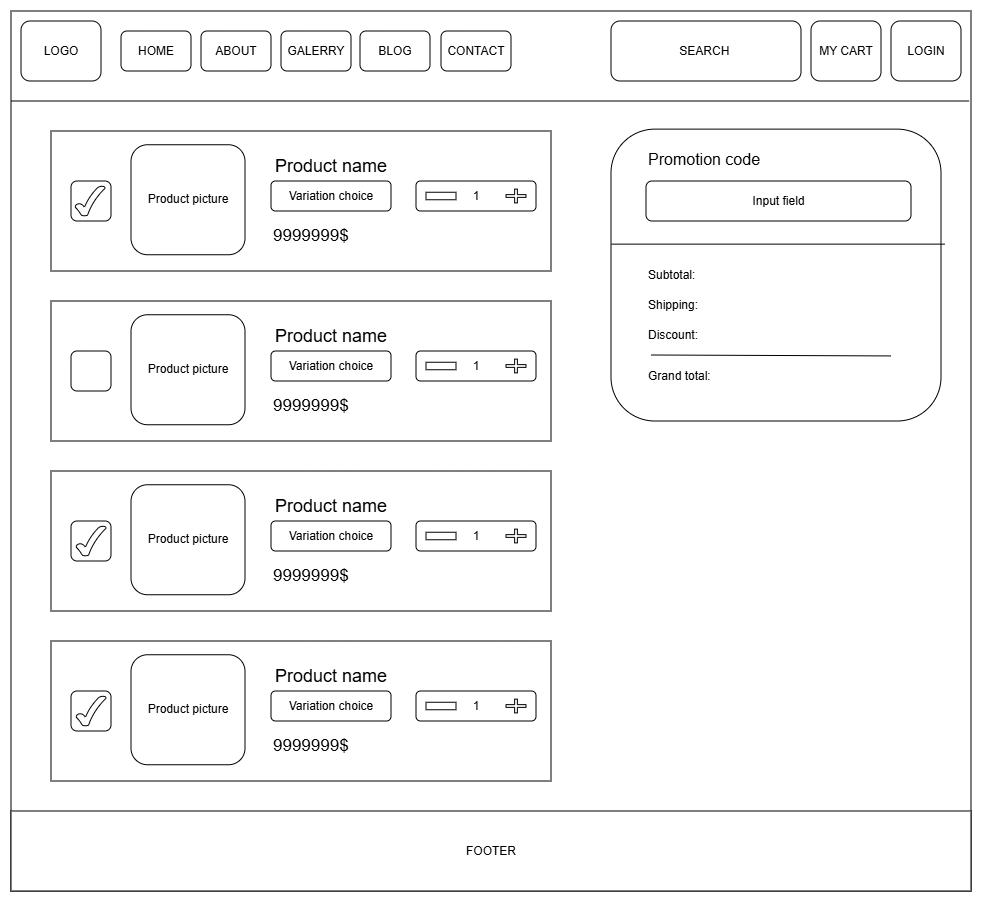
\includegraphics[width=0.91\textwidth]{VissoftIntern-MY_CART.drawio.png}
\caption{Wireframe trang giỏ hàng}
\label{fig:cart}
\end{figure}

\chapter{Bảo mật, phân quyền và vận hành}
\section{Authentication và authorization}
\begin{sloppypar}
\raggedright
JWT Bearer được kiểm tra ở backend. RBAC phân biệt Super Admin, Store Manager, Salesperson, Warehouse Staff, Dispatcher, Marketer, Accountant và CS Agent. Ngoài role, backend phải kiểm tra phạm vi store/warehouse để ngăn truy cập dữ liệu ngoài chi nhánh.
\end{sloppypar}

\section{Bảo vệ dữ liệu}
Mật khẩu lưu dưới dạng hash; token, password và dữ liệu thẻ không được ghi vào log. Dữ liệu audit nhạy cảm có thể được mã hóa trước khi lưu. Input postcode, email, điện thoại, địa chỉ, số lượng, giá và trạng thái phải được validate ở boundary. WebSocket chỉ cho phép thành viên hợp lệ của session nhận message.

\section{Rate limit và health check}
\begin{sloppypar}
\raggedright
Rate limit được áp dụng theo IP hoặc user/session trên Redis, trả HTTP 429 khi vượt ngưỡng. Các ngưỡng tham khảo là 60 request/phút cho storefront public, 300 cho POS/staff và 1000 cho admin/background service.
\end{sloppypar}
\begin{sloppypar}
\raggedright
\texttt{healthz} kiểm tra process; \texttt{readyz} kiểm tra PostgreSQL, Redis và các dependency bắt buộc.
\end{sloppypar}

\section{Audit và quan sát hệ thống}
Các sự kiện cần audit gồm thay đổi giá, cập nhật order, payment, inventory, delivery, profit và commission. Mỗi record nên có actorId, requestId, entityType, entityId, action, before, after và createdAt. Monitoring cần theo dõi latency, lỗi 4xx/5xx, lock timeout, queue retry, cache hit/miss và trạng thái readiness.

\chapter{Yêu cầu phi chức năng và tiêu chí nghiệm thu}
\begin{longtable}{P{4.2cm}P{4.0cm}P{6.0cm}}
\toprule
Nhóm & Mục tiêu & Cách kiểm chứng\\
\midrule
Tìm kiếm & Khoảng 0.2--2.0 giây ở quy mô catalog lớn & Benchmark query và API theo dữ liệu mẫu.\\
Landed cost & Sai lệch không quá 0.01 AUD/USD & Unit test công thức và test dữ liệu biên.\\
Tồn kho & Không âm và không reservation vượt capacity & Integration test với request đồng thời.\\
Route & Tối ưu 10--20 stop trong tối đa khoảng 3 giây & Test tích hợp Maps/mock và đo latency.\\
Storefront & FCP mục tiêu không quá 1.5 giây ở thị trường mục tiêu & Lighthouse/performance test.\\
Chat & Độ trễ hai chiều mục tiêu không quá 200 ms & WebSocket integration test.\\
Audit & 100\% thay đổi giá/order quan trọng có log & Kiểm tra event và database audit.\\
Payment & Không lưu dữ liệu thẻ thô, callback idempotent & Security test và replay callback test.\\
\bottomrule
\caption{Ma trận yêu cầu phi chức năng}\label{tab:nfr}\\
\end{longtable}

\section{Kịch bản nghiệm thu end-to-end}
\begin{enumerate}
  \item Đăng nhập nhân viên POS và kiểm tra role/store scope.
  \item Khách nhập postcode, nhận store phục vụ và xem giá theo store.
  \item Tạo Order Now hoặc Pre-order; kiểm tra reservation và available quantity.
  \item Nhập container; xác nhận lot FIFO, landed cost và đối chiếu pre-order.
  \item Tạo delivery booking, tối ưu route, chuyển stop qua Prepare/Shipping/Done.
  \item Xác nhận outbound FIFO, actual cost, actual profit và commission.
  \item Hủy/đổi đơn; xác nhận adjustment tồn, profit, loyalty và commission.
  \item Gửi message storefront và xác nhận đúng CSKH session nhận được.
  \item Làm gián đoạn Redis hoặc dịch vụ ngoài; xác nhận dữ liệu PostgreSQL đã commit không bị mất.
\end{enumerate}

\chapter{Kết luận thiết kế}
Đây là bản phân tích thiết kế khởi đầu cho hệ thống quản lý bán hàng đa chi nhánh. Nội dung đã phác thảo các yêu cầu nghiệp vụ, kiến trúc, dữ liệu, API, luồng xử lý và giao diện ở mức định hướng.

Trong quá trình triển khai và sử dụng thực tế, vẫn có thể phát sinh nhiều vấn đề liên quan đến dữ liệu, tích hợp, hiệu năng, bảo mật, tính nhất quán giao dịch, trải nghiệm người dùng và các trường hợp ngoại lệ nghiệp vụ. Vì vậy, tài liệu cần tiếp tục được kiểm chứng, cập nhật và hoàn thiện dựa trên kết quả triển khai, kiểm thử và phản hồi vận hành.

\end{document}
